\begin{center}
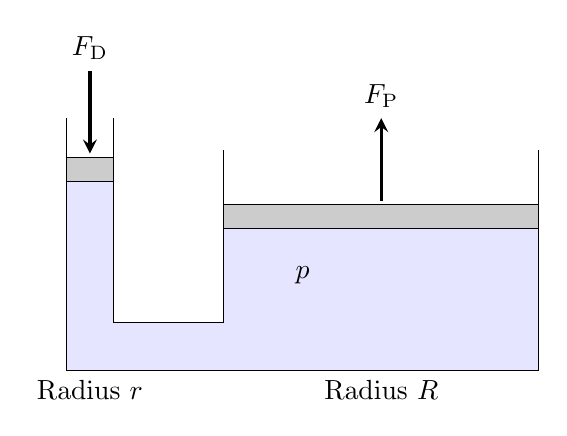
\begin{tikzpicture}[>=stealth]
 \fill[blue!10] (0,0) rectangle (6,0.6);
 \fill[blue!10] (0,0.6) rectangle (0.6,2.4);
 \fill[blue!10] (2,0.6) rectangle (6,1.8);
 \draw (0,3.2) -- (0,0) -- (6,0) -- (6,2.8);
 \draw (0.6,3.2) -- (0.6,0.6) -- (2,0.6) -- (2,2.8);
 \draw[fill=gray!40] (0,2.4) rectangle (0.6,2.7);
 \draw[fill=gray!40] (2,1.8) rectangle (6,2.1);
 \draw[->, very thick] (0.3,3.8) -- (0.3,2.75) node[pos=0, above] {$F_\mathrm{D}$};
 \draw[->, very thick] (4,2.15) -- (4,3.2) node[above] {$F_\mathrm{P}$};
 \node[below] at (0.3,0) {Radius $r$};
 \node[below] at (4,0) {Radius $R$};
 \node at (3,1.2) {$p$};
\end{tikzpicture}
\end{center}

\begin{abcliste}
\abc Der Druck in der Flüssigkeit ist überall gleich, $p = F_\mathrm{D}/(\pi r^2) = F_\mathrm{P}/(\pi R^2)$. Damit ist
\begin{align}
 F_\mathrm{D} &= \FdkF \\
   &= \Fhp\cdot\frac{\left(\rhp\right)^2}{\left(\Rhp\right)^2} \\
   &= \Fdk \approx \result{\FdkP{3}{2}}
\end{align}
\abc
\begin{align}
 p &= \phpF \\
   &= \frac{\Fhp}{\pi\cdot\left(\Rhp\right)^2} \\
   &= \php \approx \result{\phpP{6}{2}}
\end{align}
Das sind etwa \phpbP{0}{2}.
\end{abcliste}
